%%%%%%%%%%%%%%%%%%%%%%%%%%%%%%%%%%%%%%%%%
% Beamer Presentation
% LaTeX Template
% Version 1.0 (10/11/12)
%
% This template has been downloaded from:
% http://www.LaTeXTemplates.com
%
% License:
% CC BY-NC-SA 3.0 (http://creativecommons.org/licenses/by-nc-sa/3.0/)
%
%%%%%%%%%%%%%%%%%%%%%%%%%%%%%%%%%%%%%%%%%

%----------------------------------------------------------------------------------------
%	PACKAGES AND THEMES
%----------------------------------------------------------------------------------------

\documentclass[14pt]{beamer}

\mode<presentation> {

% The Beamer class slide themes
\usetheme{Madrid} %i was using this one

% Beamer class color themes

%\usecolortheme{albatross}

%\setbeamertemplate{footline} % To remove the footer line in all slides uncomment this line
%\setbeamertemplate{footline}[page number] % To replace the footer line in all slides with a simple slide count uncomment this line

%\setbeamertemplate{navigation symbols}{} % To remove the navigation symbols from the bottom of all slides uncomment this line
}

\usepackage{graphicx} % Allows including images
\usepackage{booktabs} % Allows the use of \toprule, \midrule and \bottomrule in tables
\usepackage{hyperref}
\usepackage{helvet}

%----------------------------------------------------------------------------------------
%	TITLE PAGE
%----------------------------------------------------------------------------------------

\title[-omics]{All the "-omics"} % The short title appears at the bottom of every slide, the full title is only on the title page

\author{C. Ryan Campbell} % Your name
\institute[Duke] % Your institution as it will appear on the bottom of every slide, may be shorthand to save space
{
Duke University \\ % Your institution for the title page
\medskip
\textit{c.ryan.campbell@duke.edu} % Your email address
}
\date{26 Sept 2017} % Date, can be changed to a custom date

\begin{document}

\begin{frame}
\titlepage % Print the title page as the first slide
\end{frame}

\begin{frame}
\frametitle{Overview} % Table of contents slide, comment this block out to remove it
\tableofcontents % Throughout your presentation, if you choose to use \section{} and \subsection{} commands, these will automatically be printed on this slide as an overview of your presentation
\end{frame}

%----------------------------------------------------------------------------------------
%	PRESENTATION SLIDES
%----------------------------------------------------------------------------------------

%------------------------------------------------
\section{Goals} 
%------------------------------------------------

%------------------------------------------------
\begin{frame}
\frametitle{Today's Goals}
%what students should know/learn today
\begin{itemize}
	\item What other questions can genomics answer?
	\item What technologies underlie these methods?
	\item[]
	\item Group dataset selection
\end{itemize}
\end{frame}

%------------------------------------------------
\begin{frame}
\frametitle{Methods in Context}
\begin{itemize}
	\large
	\item[] My goal is to present the methods as:
	\normalsize
	\item Biological Question
	\begin{itemize}
		\item[] (Broad enough to apply to whatever system)
	\end{itemize}
	\item Underlying NGS
	\item A paper that utilizes the method
\end{itemize}
\end{frame}

%------------------------------------------------
\section{Transcriptome}
%------------------------------------------------

%------------------------------------------------
\subsection{RNAseq}
%------------------------------------------------

%------------------------------------------------
\begin{frame}
\frametitle{RNAseq}
\begin{itemize}
	\item<+-> Biological Question:
	\begin{itemize}
		\item<+-> What genes are being expressed in a cell?
	\end{itemize}
	\item<+-> Underlying NGS:
	\begin{itemize}
		\item<+-> Illumina NGS with special library prep
	\end{itemize}
	\item<+-> Faherty. 2016. Gene Expression Profiling in the Hibernating Primate, Cheirogaleus Medius.
\end{itemize}
\end{frame}

%------------------------------------------------
\subsection{Allele Specific Expression}
%------------------------------------------------

%------------------------------------------------
\begin{frame}
\frametitle{ASE}
\begin{itemize}
	\item<+-> Allele-Specific Expression
	\item<+-> Quantification of gene expression by diploid copy
	\item<+-> Can determine effect of small-scale changes on expression
\end{itemize}
\end{frame}

%------------------------------------------------
\begin{frame}
\frametitle{ASE}
\begin{columns}
	\begin{column}{0.4\textwidth}
		\begin{itemize}
			\item<+-> Comparing haplotypes allows for detection of differences:
			\item<+-> Stop Codons
			\item<+-> SNPs
			\item<+-> TF binding sites or methylation
		\end{itemize}
		\end{column}
	\begin{column}{0.6\textwidth}
		\begin{center}
     		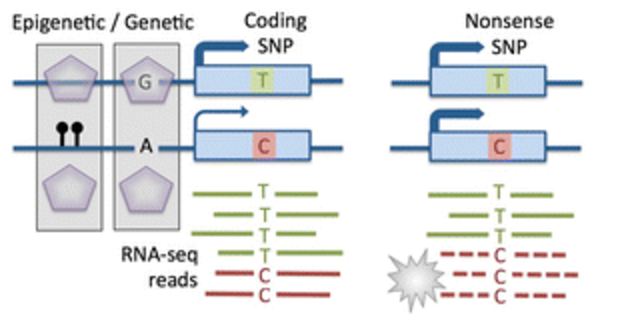
\includegraphics[width=1\textwidth]{images_20170926_ASE.png}
     	\end{center}
	\end{column}
\end{columns}
\end{frame}

%------------------------------------------------
\begin{frame}
\frametitle{ASE}
\begin{itemize}
	\item<+-> Biological Question:
	\begin{itemize}
		\item<+-> What of two dipliod gene copies are being expressed?
	\end{itemize}
	\item<+-> Underlying NGS:
	\begin{itemize}
		\item<+-> Illumina NGS with special library prep and post-processing
	\end{itemize}
	\item<+-> Lappalainen et al. 2013. Transcriptome and genome sequencing uncovers functional variation in humans.
\end{itemize}
\end{frame}

%------------------------------------------------
\subsection{IsoSeq}
%------------------------------------------------

%------------------------------------------------
\begin{frame}
\frametitle{Iso-Seq}
\begin{itemize}
	\item<+-> Isoform Sequencing
	\item<+-> Long read RNA sequencing
	\item<+-> Allows for the full transcript to be sequenced
\end{itemize}
\end{frame}

%------------------------------------------------
\begin{frame}
\frametitle{Iso-Seq}
\begin{columns}
	\begin{column}{0.5\textwidth}
		\begin{itemize}
			\item<+-> RNAseq library preparation
			\item<+-> No fragmentation and keep full transcripts
			\item<+-> Prepare and sequence on the PacBio platform
		\end{itemize}
		\end{column}
	\begin{column}{0.5\textwidth}
		\begin{center}
     		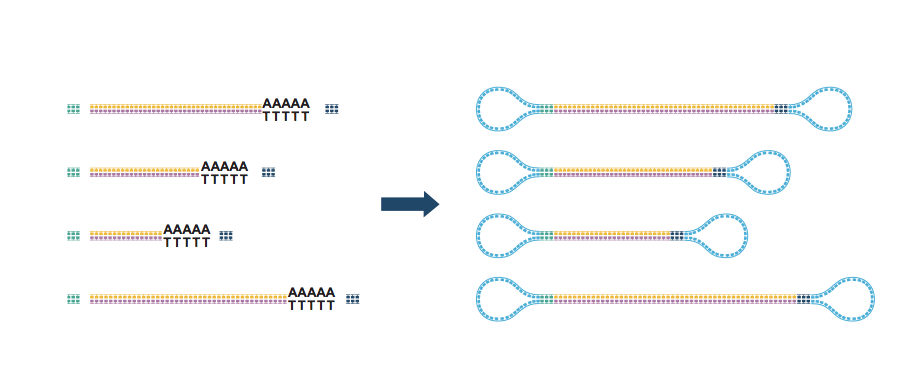
\includegraphics[width=1\textwidth]{images_20170926_isoseqprep.png}
     	\end{center}
	\end{column}
\end{columns}
\end{frame}

%------------------------------------------------
\begin{frame}
\frametitle{Iso-Seq}
\begin{columns}
	\begin{column}{0.4\textwidth}
		\begin{itemize}
			\item<+-> Get longer data
			\item<+-> Don't have to assemble full transcripts
			\item<+-> Actually ``see'' all the isoforms
		\end{itemize}
		\end{column}
	\begin{column}{0.6\textwidth}
		\begin{center}
     		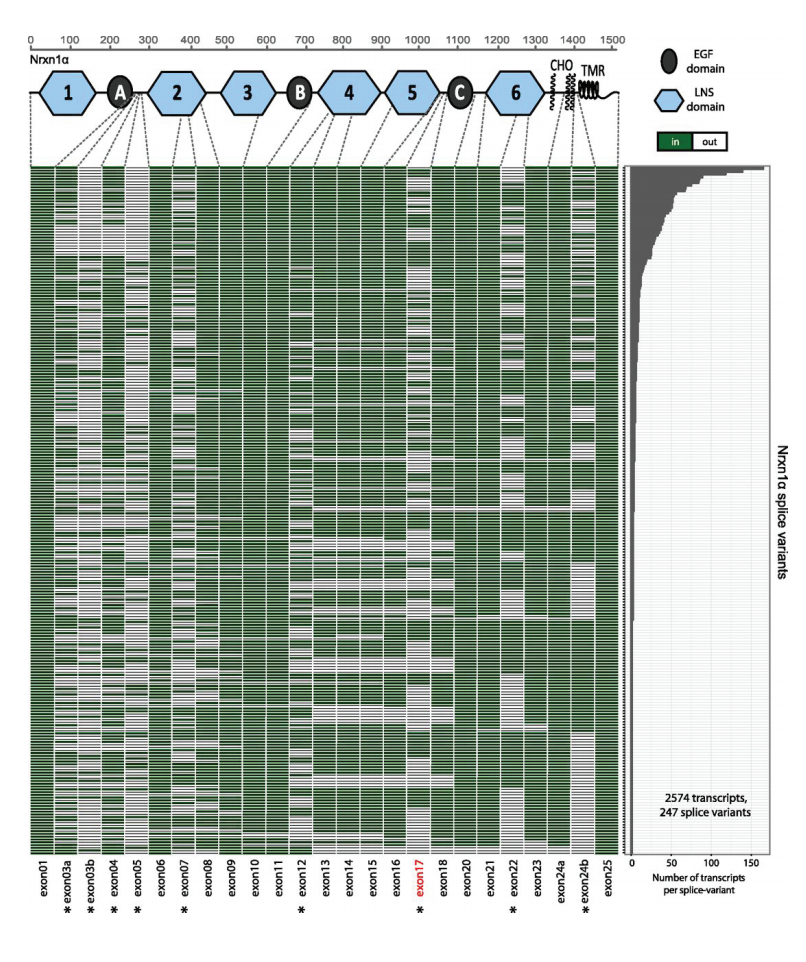
\includegraphics[width=1\textwidth]{images_20170926_isoseqout.png}
     	\end{center}
	\end{column}
\end{columns}
\end{frame}

%------------------------------------------------
\begin{frame}
\frametitle{Iso-Seq}
\begin{itemize}
	\item<+-> Biological Question:
	\begin{itemize}
		\item<+-> What isoforms of a gene are being expressed?
	\end{itemize}
	\item<+-> Underlying NGS:
	\begin{itemize}
		\item<+-> RNAseq using PacBio to sequencing whole transcripts
	\end{itemize}
	\item<+-> Cheng et al. 2017. Long-read sequencing of the coffee bean transcriptome reveals the diversity of full-length transcripts.
\end{itemize}
\end{frame}

%------------------------------------------------
\section{Microbiome}
%------------------------------------------------

%------------------------------------------------
\begin{frame}
\frametitle{Microbiome}
\begin{itemize}
	\item<+-> What is the community of microbes that live within vertebrates?
	\item<+-> Gut is most commonly studied, but there are plenty of other targets
\end{itemize}
\end{frame}

%------------------------------------------------
\begin{frame}
\frametitle{Microbiome}
\begin{itemize}
	\item<+-> Often longitudinal:
	\begin{itemize}
		\item<+-> How does this community change over a lifespan?
		\item<+-> How do antibiotics alter this community?
	\end{itemize}
	\item<+-> Also can compare across populations (diet effect)
	\item<+-> Can often tell a differnce based on lifestyle 
\end{itemize}
\end{frame}

%------------------------------------------------
\subsection{16S}
%------------------------------------------------

%------------------------------------------------
\begin{frame}
\frametitle{16S Region}
\begin{itemize}
	\item<+-> 16S is a ``barcode'' region of bacterial genomes
	\begin{itemize}
		\item<+-> Often stable (encodes ribosomal RNA molecule)
		\item<+-> Used to distinguish ``species''
	\end{itemize}
	\item<+-> The most common form of microbiome research amplifies this region
	\item<+-> Then sequencing is performed to assess the community 
\end{itemize}
\end{frame}

%------------------------------------------------
\subsection{Metagenomics}
%------------------------------------------------

%------------------------------------------------
\begin{frame}
\frametitle{Metagenomics}
\begin{itemize}
	\item<+-> Broad, non-targeted method of censusing the microbiome
	\item<+-> Gather a sample and prepare all the DNA therein for sequencing
	\item<+-> Catches everything, unbiased
	\item<+-> Categorization is often difficult
	\item<+-> Captures functional capabilities of microbiota
\end{itemize}
\end{frame}

%------------------------------------------------
\begin{frame}
\frametitle{16S v. Metagenomics}
\centerline{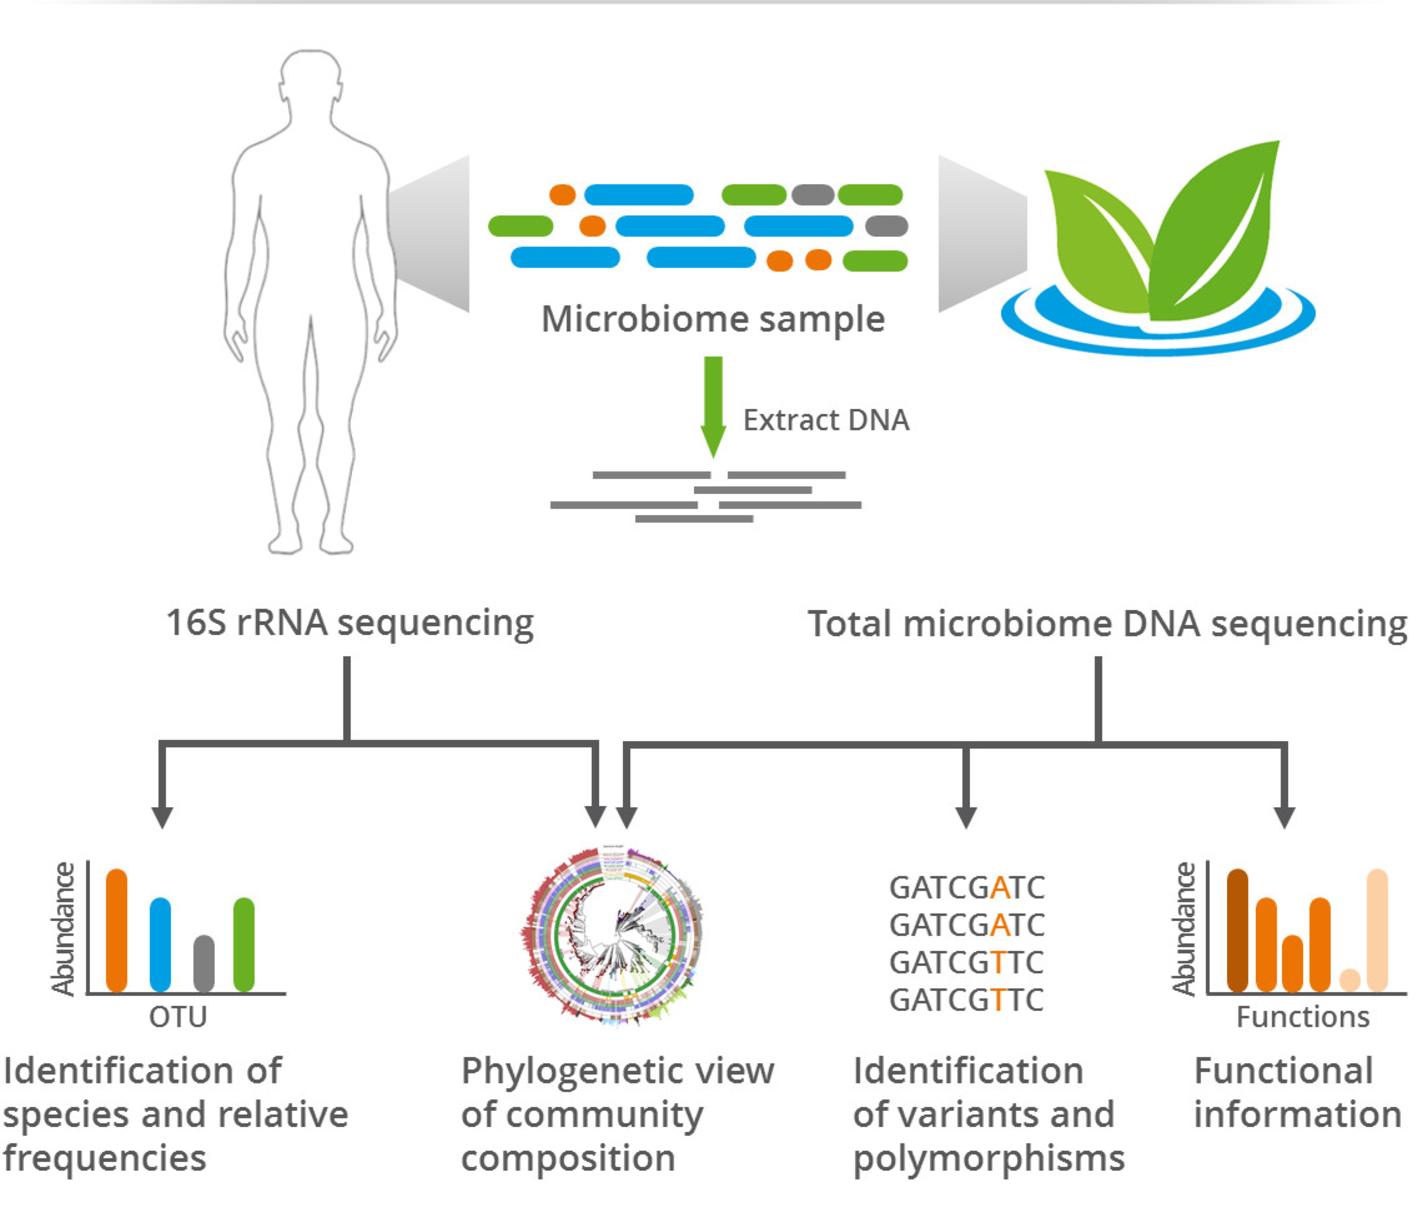
\includegraphics[width=0.8\textwidth]{images_20170926_microbiome.png}}
\end{frame}

%------------------------------------------------
\begin{frame}
\frametitle{Microbiome}
\begin{itemize}
	\item<+-> Biological Question:
	\begin{itemize}
		\item<+-> What bacteria live in the gut? 
	\end{itemize}
	\item<+-> Underlying technology:
	\begin{itemize}
		\item<+-> Illumina NGS with a narrow input (16S region) and special processing
		\item<+-> Illumina NGS with a broad input (any DNA) and special processing
	\end{itemize}
	\item<+-> Davie et al. 2014. Diet rapidly and reproducibly alters the human gut microbiome.
\end{itemize}
\end{frame}



%------------------------------------------------
\section{Epigenomics}
%------------------------------------------------

%------------------------------------------------
\begin{frame}
\frametitle{Epi-}
\begin{itemize}
	\item<+-> Epi- means?
	\item<+-> On, upon
	\item<+-> Above
\end{itemize}
\end{frame}

%------------------------------------------------
\begin{frame}
\frametitle{Epigenomics}
\begin{itemize}
	\item<+-> Changes that occur ``on'' the genome
	\item<+-> More broadly - changes that aren't encoded in the DNA
	\begin{itemize}
		\item<+-> Methylation of Cytosines
		\item<+-> Chromatin status
		\item<+-> microRNAs
	\end{itemize}
\end{itemize}
\end{frame}

%------------------------------------------------
\subsection{Methylation}
%------------------------------------------------

%------------------------------------------------
\begin{frame}
\frametitle{Methylation}
\begin{itemize}
	\item<+-> Methyl group is added to a cytosine
	\item<+-> (Adenine can too, just less common)
	\item<+-> Supresses transcription if it occurs in a gene promoter region
\end{itemize}
\end{frame}

%------------------------------------------------
\begin{frame}
\frametitle{Methylation}
\begin{columns}
	\begin{column}{0.4\textwidth}
		\begin{itemize}
			\item<+-> Often present near TE's and Genes
			\item<+-> Presence mutes TE's
			\item<+-> Absence allows gene transcription
		\end{itemize}
		\end{column}
	\begin{column}{0.6\textwidth}
		\begin{center}
     		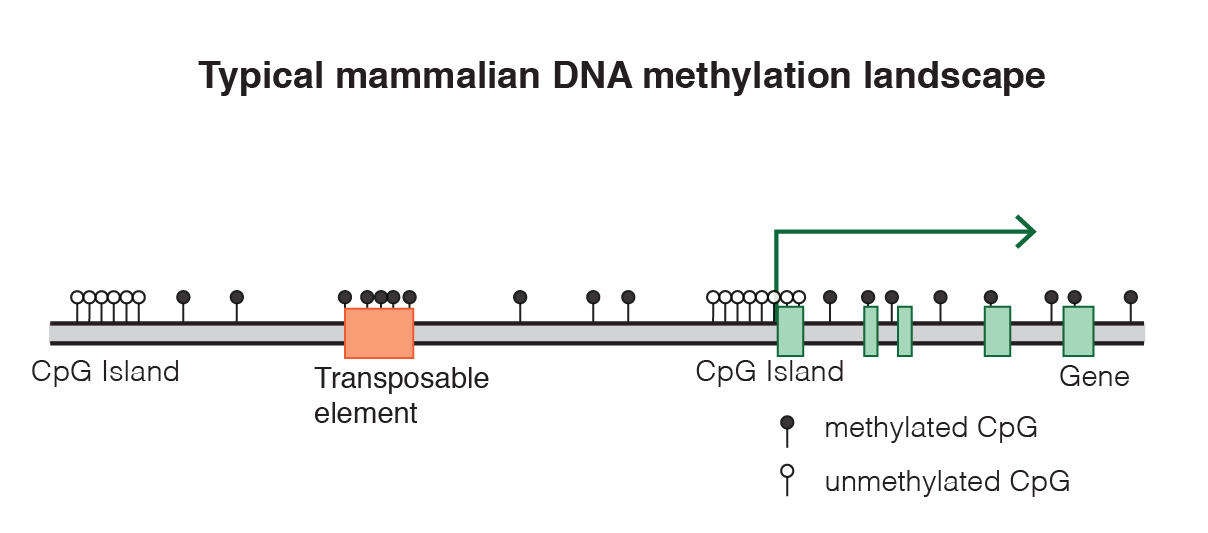
\includegraphics[width=1\textwidth]{images_20170926_methyl.png}
     	\end{center}
	\end{column}
\end{columns}
\end{frame}

%------------------------------------------------
\begin{frame}
\frametitle{Bisulfite Sequencing}
\begin{columns}
	\begin{column}{0.4\textwidth}
		\begin{itemize}
			\item<+-> Library prep converts unmethylated C's to U's
			\item<+-> Leaves methylated C's as C's
			\item<+-> Sequence to determine where methylated sites are
		\end{itemize}
		\end{column}
	\begin{column}{0.6\textwidth}
		\begin{center}
     		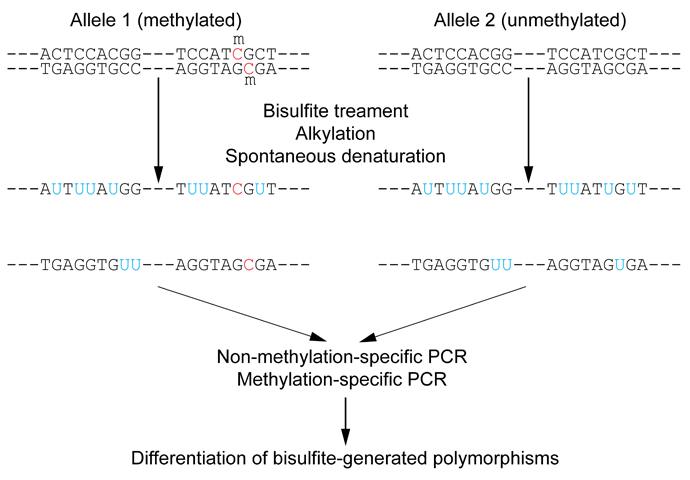
\includegraphics[width=1\textwidth]{images_20170926_bisulfite.png}
     	\end{center}
	\end{column}
\end{columns}
\end{frame}

%------------------------------------------------
\begin{frame}
\frametitle{Bisulfite Sequencing}
\begin{itemize}
	\item<+-> Biological Question:
	\begin{itemize}
		\item<+-> Which bases in the genome are methylated?
	\end{itemize}
	\item<+-> Underlying NGS:
	\begin{itemize}
		\item<+-> Illumina NGS with bisulfite conversion
	\end{itemize}
	\item<+-> Lea et al. 2016. Resource base influences genome‐wide DNA methylation levels in wild baboons (Papio cynocephalus).
\end{itemize}
\end{frame}

%------------------------------------------------
\subsection{ATAC-seq}
%------------------------------------------------

%------------------------------------------------
\begin{frame}
\frametitle{ATAC-seq}
\begin{itemize}
	\item<+-> Assay for Transposase-Accessible Chromatin using sequencing
	\item<+->  
\end{itemize}
\end{frame}

%------------------------------------------------
\begin{frame}
\frametitle{ATAC-seq}
\begin{columns}
	\begin{column}{0.6\textwidth}
		\begin{itemize}
			\item<+-> Transposase (green)
			\item<+-> Sequencing adaptors (red and blue)
			\item<+-> Inserts only in regions of open chromatin, between nucleosomes
		\end{itemize}
		\end{column}
	\begin{column}{0.4\textwidth}
		\begin{center}
     		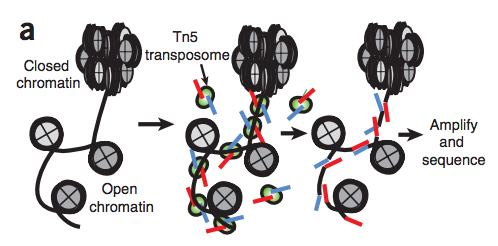
\includegraphics[width=1\textwidth]{images_20170926_ATACsmall.png}
     	\end{center}
	\end{column}
\end{columns}
\end{frame}

%------------------------------------------------
\begin{frame}
\frametitle{ATAC-seq}
\centerline{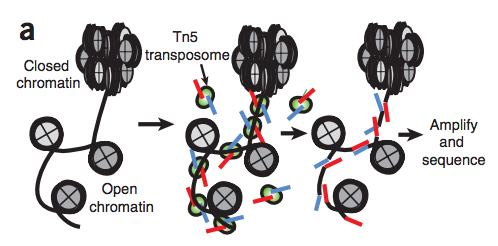
\includegraphics[width=0.95\textwidth]{images_20170926_ATACsmall.png}}
\end{frame}

%------------------------------------------------
\begin{frame}
\frametitle{ATAC-seq Results}
\centerline{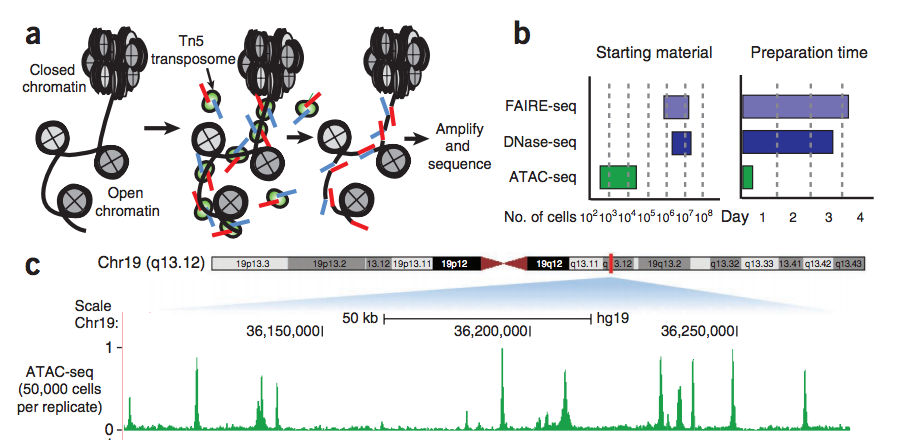
\includegraphics[width=0.95\textwidth]{images_20170926_ATAClarge.png}}
\end{frame}

%------------------------------------------------
\begin{frame}
\frametitle{ATAC-seq}
\begin{itemize}
	\item<+-> Biological Question:
	\begin{itemize}
		\item<+-> Which regions of the genome are accessible?
	\end{itemize}
	\item<+-> Underlying NGS:
	\begin{itemize}
		\item<+-> Cutting open regions out and prep for Illumina NGS
	\end{itemize}
	\item<+-> Ackerman et al. 2016. Integration of ATAC-seq and RNA-seq identifies human alpha cell and beta cell signature genes.
\end{itemize}
\end{frame}

%------------------------------------------------
\section{Non-Epigenomics}
%------------------------------------------------

%------------------------------------------------
\begin{frame}
\frametitle{Non-Epigenomics}
\begin{itemize}
	\item<+-> There are other measures ``above'' the DNA-level
	\item<+-> However, they're not heritable
	\item<+-> So not technically epigenetic
	\item<+-> (But the methods are very similar)
\end{itemize}
\end{frame}

%------------------------------------------------
\subsection{CHIPseq}
%------------------------------------------------

%------------------------------------------------
\begin{frame}
\frametitle{CHIPseq}
\begin{itemize}
	\item<+-> Chromatin Immunoprecipitation sequencing
	\item<+-> Capture DNA that is currently bound to a protein
	\item<+-> Works for any protein of interest
	\item<+-> Often used in Transcription Factor work
\end{itemize}
\end{frame}

%------------------------------------------------
\begin{frame}
\frametitle{CHIPseq}
\begin{columns}
	\begin{column}{0.6\textwidth}
		\begin{itemize}
			\item<+-> Fix protein to DNA
			\item<+-> Break up genome
			\item<+-> Capture and sequence only DNA that is attached to protein
		\end{itemize}
		\end{column}
	\begin{column}{0.4\textwidth}
		\begin{center}
     		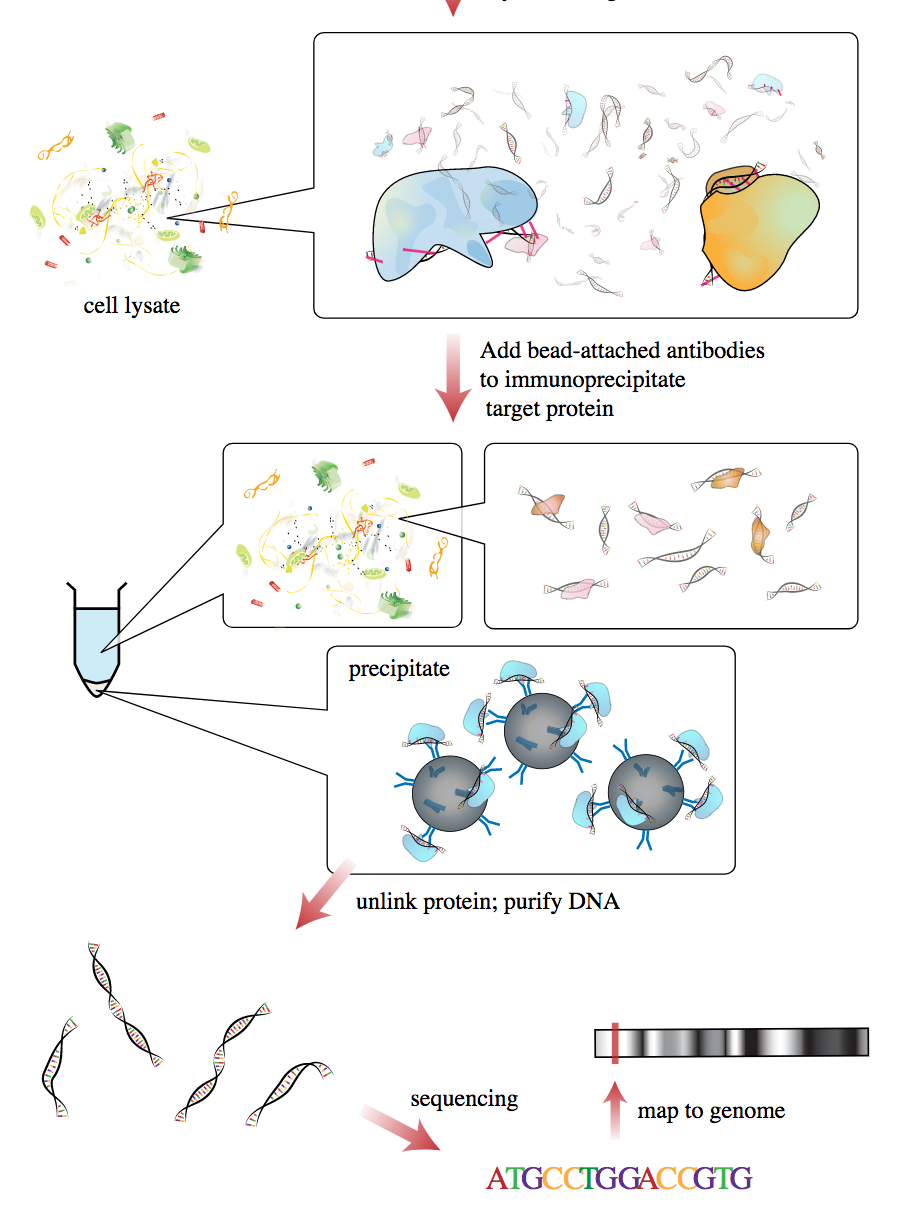
\includegraphics[width=1\textwidth]{images_20170926_CHIP.png}
     	\end{center}
	\end{column}
\end{columns}
\end{frame}

%------------------------------------------------
\begin{frame}
\frametitle{CHIPseq}
\begin{itemize}
	\item<+-> Biological Question:
	\begin{itemize}
		\item<+-> Where is a given protein bound to DNA?
	\end{itemize}
	\item<+-> Underlying NGS:
	\begin{itemize}
		\item<+-> Protein pulldown and library prep for Illumina NGS
	\end{itemize}
	\item<+-> Schmidt. 2010. Five-Vertebrate ChIP-seq Reveals the Evolutionary Dynamics of Transcription Factor Binding.
\end{itemize}
\end{frame}

%------------------------------------------------
\section{Project Data Selction}
%------------------------------------------------

%------------------------------------------------
%%UNCOMMENT
\begin{frame}
\frametitle{Get with your Groups:}
	\begin{itemize}
	\item Jennifer, Nayib, Chris
	\item Austin, Alan, Raymond - flies and bacteria
	\item Othmane, Kevin, Alvin
	\item Helena, Jake, Rahul - flies and devo
	\item Hank, Sisi, Joy
	\end{itemize}
\end{frame}

%------------------------------------------------
\begin{frame}
	\begin{itemize}
		\item {\Large Today's Tasks:}
		\item Meet with your group
		\item Discuss possible datasets
		\item Settle on a preference and clear it with me
		\item Find sra link for Thursday
	\end{itemize}
\end{frame}


%------------------------------------------------
\begin{frame}
\Huge{\centerline{The End}}
\end{frame}

%----------------------------------------------------------------------------------------

\end{document} 